\documentclass{article}%
\usepackage[T1]{fontenc}%
\usepackage[utf8]{inputenc}%
\usepackage{lmodern}%
\usepackage{textcomp}%
\usepackage{lastpage}%
\usepackage[head=40pt,margin=0.5in,bottom=0.6in]{geometry}%
\usepackage{graphicx}%
%
\title{\textbf{Denuncian que el ELN ocupa áreas de Lara y Falcón}}%
\author{SANDRA GUERRERO | Sguerrero@el{-}nacional.com}%
\date{23/11/2018}%
%
\begin{document}%
\normalsize%
\maketitle%
\textbf{URL: }%
http://www.el{-}nacional.com/noticias/sucesos/denuncian{-}que{-}eln{-}ocupa{-}areas{-}lara{-}falcon\_260780\newline%
%
\textbf{Periodico: }%
EN, %
ID: %
260780, %
Seccion: %
Sucesos\newline%
%
\textbf{Palabras Claves: }%
Falcón, Lara, Sucesos\newline%
%
\textbf{Derecho: }%
CONTEXTO%
, Otros Derechos: %
NO\_TIENE%
, Sub Derechos: %
NO\_TIENE%
\newline%
%
\textbf{EP: }%
NO\newline%
\newline%
%
\textbf{\textit{Javier Tarazona, director general de la ONG, entregó en el Ministerio Público fotografías satelitales de los asentamientos guerrilleros donde se encuentran}}%
\newline%
\newline%
%
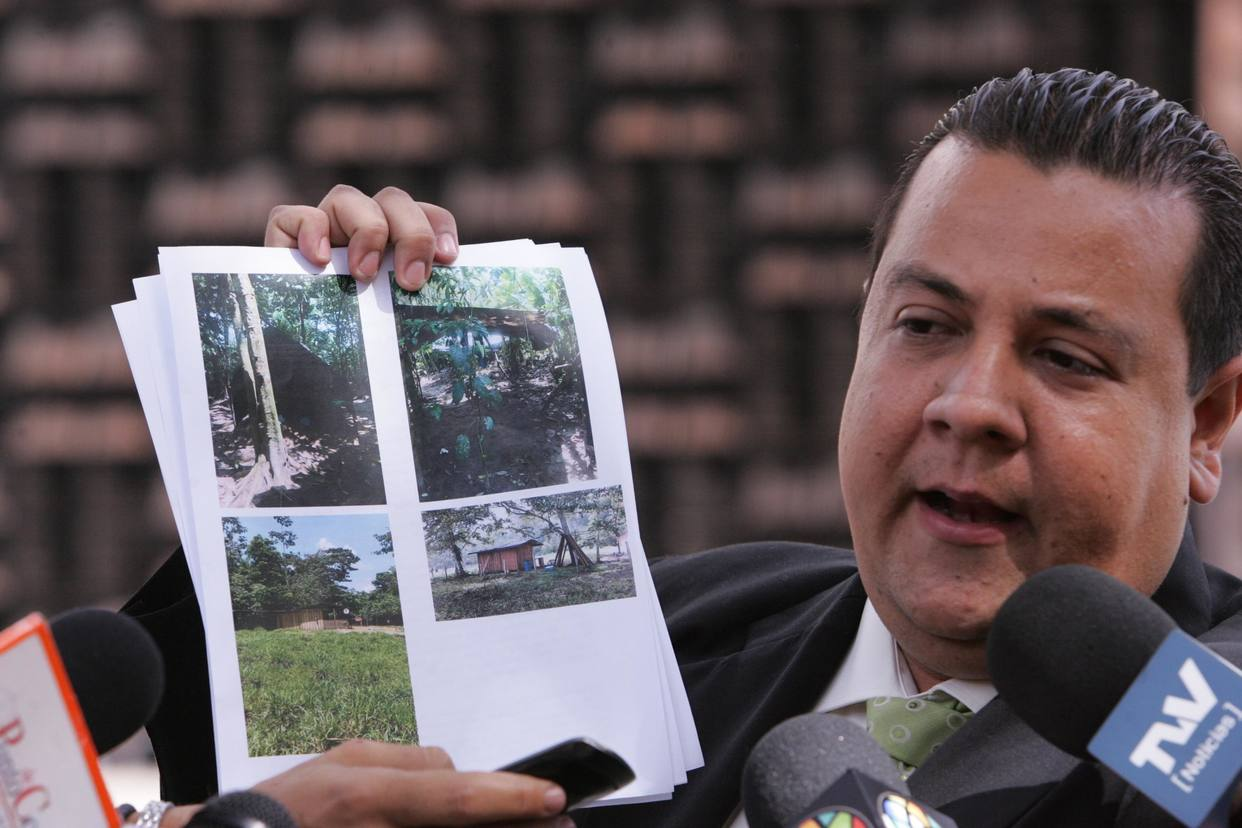
\includegraphics[width=300px]{139.jpg}%
\newline%
%
Javier Tarazona, director de FundaRedes, entregó ayer en el Ministerio Público la denuncia, acompañada con pruebas, de que la guerrilla colombiana, concretamente el ELN, ocupa parte de territorios en los estados Lara y Falcón. En Lara, los asentamientos están en Moroturo, San Miguel, Siquisiqui y Urdaneta; mientras que en Falcón, los irregulares ocupan Los Alambiques, la Sierra de San Luis y Churuguara.%
\newline%
%
Tarazona explicó que en esas zonas el ELN actúa al margen de la ley “mediante el microtráfico, narcotráfico, extorsión a ciudadanos, además del contrabando de minerales como oro, diamante y coltán hacia las costas de Falcón con destino a las islas de Aruba, Curazao y Bonaire. “Estas son utilizadas como estrategia geopolítica”, explicó Tarazona.%
\newline%
%
Agregó que en más de 18 ocasiones ha formulado denuncias relacionadas con la actividad de la guerrilla en 14 estados del país y la Fiscalía sigue guardando silencio.%
\newline%
%
Tarazona dijo que ve con mucha preocupación lo que está ocurriendo en el territorio nacional, donde además del ELN actúan otros grupos irregulares provenientes del vecino país. Igualmente manifestó que esas organizaciones cuentan con emisoras de radio y revistas, mediante las cuales reclutan y adoctrinan niños.%
\newline%
%
El director de FundaRedes dijo que entregaría en el Ministerio Público las fotografías satelitales de cómo opera el Ejército de Liberación Nacional de forma temporal y permanente en los estados Lara y Falcón.%
\newline%
%
Indicó que la entrega de esas evidencias tiene como fin que las autoridades, junto con las Fuerzas Armadas, inicien la investigación del grupo irregular en esos dos estados.%
\newline%
%
En cuanto a las 18 denuncias formuladas ante el Ministerio Público por esa organización, indicó: “Solo hemos encontrado silencio, no ha habido respuesta”. Reiteró que la guerrilla colombiana no solo ocupa las fronteras de Venezuela, sino que también está en el oriente, sur y centro del país “para un mejor control político y social con al anuencia del gobierno”, dijo.%
\newline%
%
Al referirse a la muerte de integrantes de las FANB a manos de los grupos irregulares del vecino país, Tarazona manifestó que tienen conocimiento de que son cinco los militares ultimados este año. Uno en Zulia, dos murieron por la explosión de una mina y además de los tres integrantes de la GNB muertos en Amazonas, hace unas semanas. “Esto, con la complicidad de las autoridades venezolanas”, explicó.%
\newline%
%
La investigación que adelanta FundaRedes indica que en el país actúan 10 grupos de irregulares, “además del ELN y las FARC, Los Rastrojos, Urebeños, Botas de Cuero, Frente Bolivariano de Liberación y el Colectivo del Pueblo que lo dirige el ELN.%
\newline%
%
Tarazona criticó la presencia de Rodrigo Granda, quien hace días se presentó en el país. “Vino a hablar de paz, un hombre que tiene las manos manchadas de sangre”, aseguró.%
\newline%
%
ElDato%
\newline%
%
En un operativo de la policía y de la Fiscalía colombiana apresaron a seis autores materiales e intelectuales del plagio del menor Cristo José, hijo de un alcalde, dijo el presidente Iván Duque. La captura fue en los límites con Venezuela donde el 3 de octubre ocurrió el secuestro.%
\newline%
%
\end{document}